\documentclass[runningheads]{llncs}
\usepackage[T1]{fontenc}
\usepackage{lmodern}
\usepackage{graphicx}
\usepackage{amsmath,amssymb}
\usepackage{booktabs}
\usepackage{array}
\usepackage{microtype}
\usepackage{xcolor}
\usepackage[hidelinks]{hyperref}
\newcommand{\R}{\mathbb{R}}
\newcommand{\B}{\mathcal{B}}
\renewcommand{\paragraph}[1]{\smallskip\noindent\textbf{#1}\ }

% Every number in this paper comes from a stored result file; see SOURCES.md.

\begin{document}
\title{TRIAD: Bundle Completion from Shared Relations}
\titlerunning{TRIAD: Bundle Completion from Shared Relations}
\author{Ajit \and Soumen}
\authorrunning{Ajit and Soumen}
\institute{}
\maketitle

% =====================================================================================================================
\begin{abstract}
Bundle completion asks for the missing items of a partial bundle, such as the rest of an outfit or the next songs of
a playlist. Recent neural models learn a representation for every item, yet most items occur in only a few bundles,
and on identical splits these models fall below simple scorers that read co-occurrence and content directly. We argue
that bundle completion rests on relations between items that are shared across the catalogue: what goes with what,
whether labels agree, and what has been bundled together. It does not rest on knowing each item. In the test
queries of seven datasets, 43\% to 77\% contain a seed that no training bundle holds, and in outfits the missing item
almost never shares a seed's category, so plain similarity finds almost nothing. Following this principle, TRIAD learns one scoring
function over item relations, with no item identities: a learned content map over item features and the
features of past partners, co-occurrence with learned popularity discounts, a learned rule for shared labels, and a
per-query gate. Its parameter space contains the standard heuristics as special settings, it starts at one of them,
and it is trained with each bundle removed from its own counts. With 74,136 parameters at any catalogue size, TRIAD
is significantly ahead of the best validation-tuned simple scorer on all seven datasets and scores 13\% to 130\%
above CLHE.
\keywords{bundle completion \and recommender systems \and item relations \and evaluation}
\end{abstract}

% =====================================================================================================================
\section{Introduction}
\label{sec:intro}

A bundle is a set of items used together: an outfit of a top, trousers and shoes; a playlist built around a few
artists; a set of products bought for one purpose. A merchandiser or a listener often picks a few items and asks the
system for the rest. This is \emph{bundle completion}: given some items of a bundle (the \emph{seeds}), rank the
catalogue so that the missing items come first (Fig.~\ref{fig:intro}a) \cite{clhe,ramen}. The query is a set of
items, not a user.

\begin{figure}[tb]
\centering
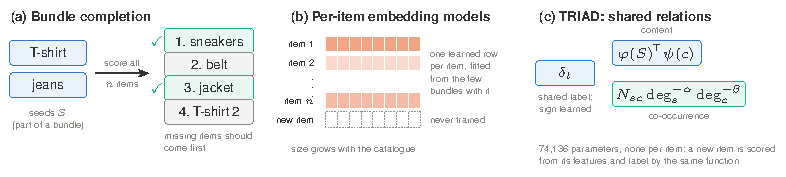
\includegraphics[width=.92\textwidth]{figs/fig1.pdf}
\caption{(a) Bundle completion ranks every catalogue item for a partial bundle. (b) Per-item models store part of
their knowledge in one learned row per item, fitted from the few bundles that contain it. (c) TRIAD learns relations
shared by all items: between item features, over labels and over co-occurrence counts.}
\label{fig:intro}
\end{figure}

\paragraph{The principle.} We argue that completing a bundle depends on \emph{relations between items} that hold
across the whole catalogue: which kinds of items go together, whether a shared category or artist is evidence for or
against a candidate, and how often items have been bundled before, discounted for items that are bundled with
everything. It does not depend on knowing each item individually. A relation can be learned from every training
bundle at once, whatever items the bundle contains; a representation of one item can be learned only from the few
bundles that contain it.

\paragraph{What existing models do.} Recent bundle models, such as CLHE \cite{clhe} and RaMen \cite{ramen}, treat
completion as representation learning (Section~\ref{sec:related}). Most of their parameters are rows of per-item
tables (Fig.~\ref{fig:intro}b), so the model grows with the catalogue, and each row is fitted only from the few
bundles that contain its item. Neither paper compares with a co-occurrence or neighbourhood method, which reads
relations between items directly, so it is open whether a representation per item is needed at all.

\begin{figure}[tb]
\centering
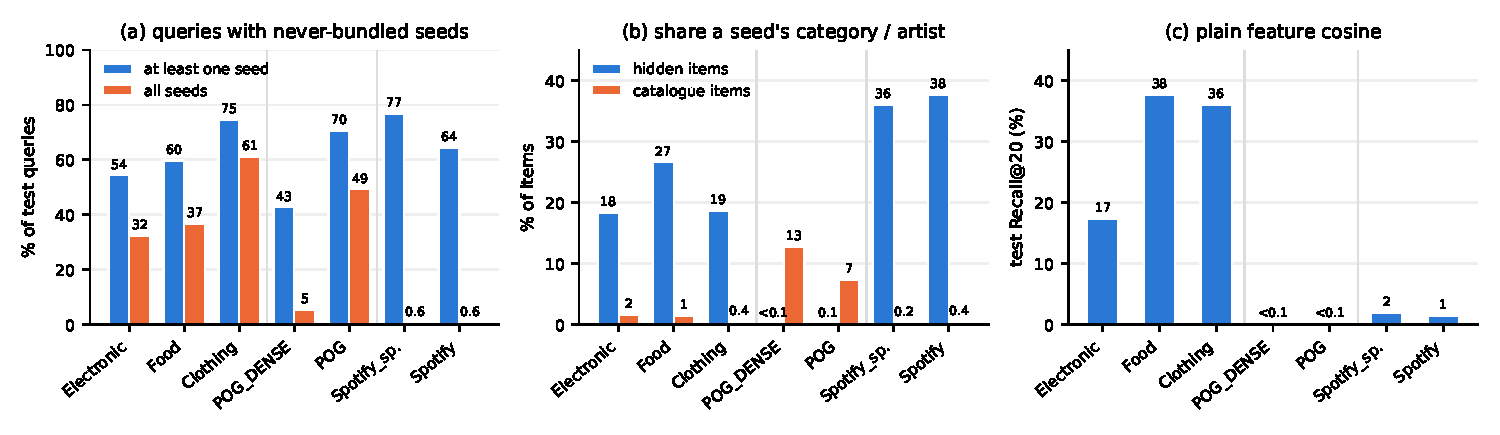
\includegraphics[width=\textwidth]{figs/data_properties.pdf}
\caption{Two properties of the data, on the clean test queries. (a) Share of queries in which
at least one seed, or every seed, occurs in no training bundle. (b) Per query, the share of hidden items whose label
(category; artist on Spotify) is among the seeds' labels, and the same share among all non-seed catalogue items, each
averaged over queries. (c) Recall@20 when the candidates
are ranked by plain feature cosine to the seeds.}
\label{fig:data}
\end{figure}

\paragraph{Why relations.} Two properties of bundle data point to relations (Fig.~\ref{fig:data}). (i) \emph{Bundle
data is sparse.} Most items occur in only a few bundles and new items keep arriving, so a query often contains items
that no training bundle holds; on most datasets this is true of most test queries, and on some, of every seed in many
of them (Fig.~\ref{fig:data}a). A per-item representation has nothing to learn from for such items; a relation over
their features and labels still applies. (ii) \emph{What goes together is not always what is similar.} In e-commerce
and playlists the missing item often shares a seed's category or artist, and items that look like the seeds are good
candidates. In outfits the missing item almost never shares a seed's category, and ranking by feature similarity finds
almost none of them (Fig.~\ref{fig:data}b,c): an outfit is completed by trousers or shoes, not by a second top. Which
relation holds depends on the domain, so it has to be learned rather than fixed.

\paragraph{Our approach.} TRIAD learns one scoring function over item relations, shared by all items
(Fig.~\ref{fig:intro}c). It combines a learned content map over item features and partner histories (the features
of the items an item was bundled with), co-occurrence with learned popularity discounts, a learned rule for shared
labels and a popularity prior, weighted per query by a gate. No parameter belongs to an item. The standard heuristics
(content cosine, cosine-normalized co-occurrence, popularity discounts, same-label rules, popularity priors) are
special settings of its parameters, and training starts at one of them. Each training bundle is removed from its own
counts while it is scored, so a model that uses counts as inputs never sees the answer.

\paragraph{Contributions.}
\begin{itemize}
\item \textbf{We identify the structure bundle completion rests on:} relations between items shared across the
catalogue, not per-item identities, and show it in the data: many queries hold never-bundled items, and complements are
not similar items.
\item \textbf{We propose TRIAD,} a model of item relations with no item identities. Its score is a learnable family
that contains the standard heuristics; it starts at one of them, and it is trained without leakage through
leave-one-out counts.
\item \textbf{TRIAD is small and accurate.} Its size does not depend on the catalogue. It is significantly ahead of
the best validation-tuned simple scorer on all seven datasets and well above CLHE and RaMen on identical splits. Its
learned parameters show what each domain relies on.
\end{itemize}

% =====================================================================================================================
\section{Related Work}
\label{sec:related}

\paragraph{From recommending bundles to completing them.} Work on bundles began with users. Bundle recommendation
ranks existing bundles for a user, for example by propagating signals over a user--bundle--item graph \cite{bgcn} or
by contrasting a bundle-level and an item-level view of the user's preferences \cite{crosscbr}. Personalized bundle
generation goes one step further and creates new bundles for a user, as a personalized list of bundles \cite{bgn} or as
an outfit assembled piece by piece \cite{pog}; generative models even draw the missing pieces of an outfit as new
images \cite{fashiondpo}. Bundle construction, the task we study, removes the user: the query is a partial bundle, and
the system must find the catalogue items that complete it \cite{clhe}. Without a user to describe, the
only evidence is the seeds themselves, their features and labels, and the bundles seen in training. The question is
how that evidence should be turned into a score.

\paragraph{Completion as representation learning.} The prevailing answer is to learn a rich representation of every
item and to match candidates against a pooled representation of the seeds. CLHE \cite{clhe} combines multimodal
features with item-level user feedback in a hierarchical encoder and adds contrastive losses at the item and the
bundle level. RaMen \cite{ramen} enriches each item with an item--item graph and a hypergraph of latent intents, and
Caro \cite{caro} strengthens item representations through category-wise and cross-modality learning. General set
models follow the same pattern: DeepSets \cite{deepsets} and the Set Transformer \cite{settransformer} pool learned
item embeddings, and basket completion with determinantal point processes learns a low-rank embedding for every item
\cite{gartrell2017}. Large language models have also been prompted to assemble bundles \cite{adabundle}, or fine-tuned
to pick the missing item from a short candidate list \cite{bundlemllm}. Generative models build the bundle as a set:
DDBC \cite{ddbc} encodes each item as a short sequence of discrete codes and fills the unknown slots by masked
diffusion, and NonMBB \cite{nonmbb} gives the known and unknown slots different noise schedules. These models
differ in architecture, but they share one design: much of what they know is stored per item and fitted from the
bundles that contain that item, which in bundle data are few (Fig.~\ref{fig:data}a). Their published comparisons are
made among such models, and the methods of the next paragraph are left out.

\paragraph{Relations read directly.} A second line of work skips item representations and scores candidates from
item--item relations computed on the training data. ItemKNN \cite{sarwar2001} uses normalized co-occurrence, RP3$\beta$
\cite{rp3beta} a random walk with a popularity penalty, EASE \cite{steck2019} a closed-form item--item regression,
LINK \cite{link} the same regression refined with multi-hop relations and pulled towards a neural model's predictions,
and graph filters \cite{gfcf,sgfcf} a smoothed co-occurrence graph. Once tuned, such methods match or beat many neural
recommenders \cite{dacrema,rendle2020}, while latent-factor models \cite{hu2008,bpr,lightgcn} again learn one
embedding per item. The relation methods have one limitation that motivates our work: each fixes its choices by hand,
for instance how strongly popular items are discounted, whether a shared category counts, and whether a candidate
should look like the seeds. TRIAD keeps their premise, scoring from relations, but turns these choices into
parameters that are learned per domain and that start at the hand-set values.

\paragraph{Complements are not look-alikes.} A simple way to use item content is to rank candidates by their
similarity to the seeds, as the content baselines in Section~\ref{sec:setup} do. This assumes that the missing item
looks like the items already in the bundle, which holds for some bundles but not for others. Product networks
distinguish substitutes, which resemble each other, from complements, which are bought together but differ
\cite{mcauley}. An outfit is a set of different pieces \cite{han2017}, and whether two pieces go together depends on
the pair of item types involved \cite{vasileva2018}. Our datasets show the same split (Fig.~\ref{fig:data}b,c),
which is why TRIAD's content map starts at similarity and is learned, and why the effect of a shared label is
learned too, as a bonus or a penalty.

\paragraph{Leakage.} Finally, a model that learns from statistics of the training data must not see the answer
inside those statistics: training on counts that include the example being scored leaks its label
\cite{kapoor2023}. TRIAD therefore removes each training bundle from its own counts while it is scored.

% =====================================================================================================================
\section{Problem Formulation}
\label{sec:problem}

\paragraph{Items, bundles and content.} Let $\mathcal{I}=\{1,\dots,n\}$ be the catalogue. A bundle is a set
$b\subseteq\mathcal{I}$ of at least two distinct items, without order, and bundle membership is recorded in the
bundle--item matrix $Y\in\{0,1\}^{|\mathcal{Y}|\times n}$ over the collection of bundles $\mathcal{Y}$, with
$Y_{b,i}=1$ if $i\in b$. Each item $i$ carries content: a text, such as its title or description, and, where
available, a media input, an image or an audio clip. Pretrained encoders turn the content into a feature vector
$x_i\in\R^{d}$ of unit length (Section~\ref{sec:features}), and $X\in\R^{n\times d}$ stacks these vectors. Item $i$ also
has a label $g_l(i)$ at each label level $l$, such as its category, or its artist and its album. Unlike
\cite{clhe,ramen}, we use no user--item interactions: bundles and item content are the only inputs.

\paragraph{Bundle completion.} The bundles are split into training bundles $\B$ and held-out bundles. For a held-out
bundle $b$, a non-empty strict subset $S\subset b$, the \emph{seeds} or partial bundle, is given, and the remaining
items $T=b\setminus S$ are hidden. The task is to recover $T$: given $S$, $X$, the labels and $\B$, rank every item
outside $S$ so that the items of $T$ come first. We solve it by learning a scoring function $s_\Theta(c\mid S)$ for
every candidate $c\in\mathcal{I}\setminus S$; the $K$ highest-scoring candidates are the prediction.

\paragraph{Statistics of the training bundles.} With $Y_{\B}$ the rows of $Y$ for the training bundles, the
co-occurrence matrix is $N=Y_{\B}^\top Y_{\B}$ with its diagonal set to zero, so $N_{sc}$ counts the training bundles
that hold both $s$ and $c$. The frequency $f_c$, the number of training bundles that hold $c$, is the diagonal of
$Y_{\B}^\top Y_{\B}$, and the degree is $\deg_c=\sum_s N_{sc}$. An item that occurs in no training bundle has $f_c=0$ and no co-occurrence, so only its content and labels describe
it; such items occur both among the seeds and among the hidden items.

% =====================================================================================================================
\section{TRIAD}
\label{sec:method}

TRIAD is a choice of the scoring function $s_\Theta$ of Section~\ref{sec:problem}. Its design starts from the simple
scorers that work well on this task (Section~\ref{sec:related}): content similarity, co-occurrence counts, shared
labels and a popularity prior. Each of them fixes a choice by hand, such as similarity as the relation between
features, a fixed popularity discount or a fixed bonus for a shared label. TRIAD keeps their inputs and learns these
choices, so each simple scorer is a special setting of its parameters, and we name this setting for each part below.
Its functions are shared by all items, so its size does not depend on the catalogue. We first give the overall score,
then the item features, the three terms and the gate, and finally the loss and its optimization.

\subsection{The Score}

For a query with seeds $S$, every candidate $c$ gets the score
\begin{equation}
s_\Theta(c\mid S)=w_C(S)\,\widehat{C}(S,c)+\textstyle\sum_l w_l(S)\,\widehat{L}_l(S,c)+w_G(S)\,\widehat{G}(S,c).
\label{eq:score}
\end{equation}
The three terms answer three questions: does $c$ fit what the seeds look like and what they were bundled with
(content $C$); does $c$ share a category, artist or album with the seeds (labels $L_l$, one per label level); and was
$c$ bundled with the seeds, and how popular is it (graph $G$). The terms have different scales, and their scales vary
from query to query, so each term is divided by its largest absolute value over the catalogue for this query,
$\widehat{Q}(S,c)=Q(S,c)/\max_{c'}|Q(S,c')|$. A gate $w(S)$ then weights the terms per query (Fig.~\ref{fig:arch}).
Several parts use a small two-layer network, which we write $\phi(x)=W_2\,\sigma(W_1x+b_1)+b_2$ with $\sigma$ the
GELU; each $\phi$ has its own weights.

\begin{figure}[tbp]
\centering
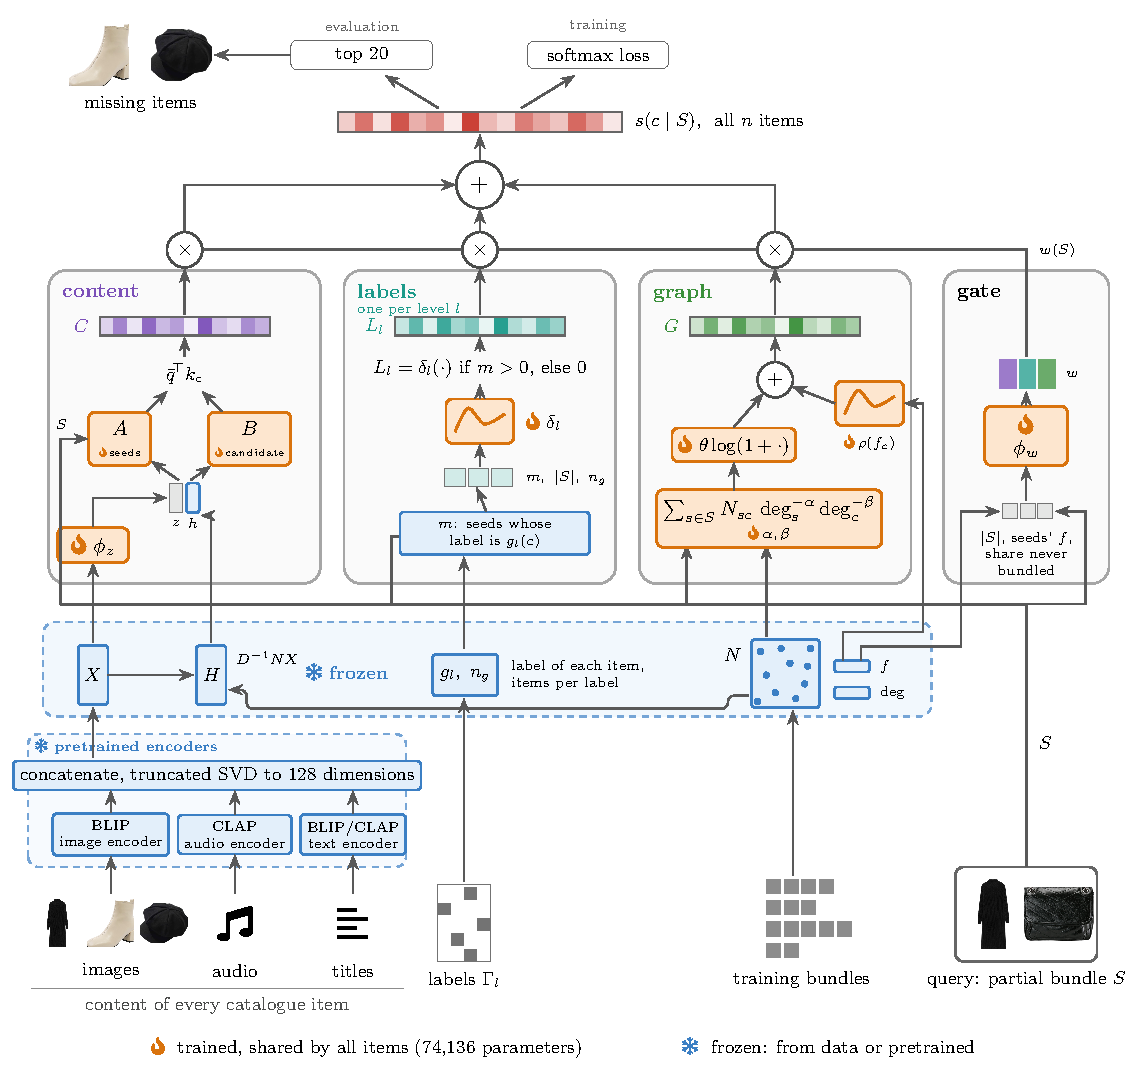
\includegraphics[width=\textwidth]{figs/architecture.pdf}
\caption{TRIAD. Item content, labels and training bundles feed the content, label and graph terms; the gate weights
them by the query, and the weighted sum scores every catalogue item.}
\label{fig:arch}
\end{figure}

\subsection{Item Features}
\label{sec:features}

TRIAD reads the content of an item (Section~\ref{sec:problem}) through a fixed feature vector. A text encoder $E_t$
and a media encoder $E_m$ from the same pretrained model, not trained further, embed the text $t_i$ and the media
input $m_i$ of item $i$, and the two embeddings are scaled to unit length and concatenated, so that each modality counts equally:
\begin{equation}
e_i=\Big[\,\frac{E_m(m_i)}{\lVert E_m(m_i)\rVert}\,;\,\frac{E_t(t_i)}{\lVert E_t(t_i)\rVert}\,\Big]\in\R^{d_m+d_t}.
\end{equation}
Stacking the $e_i$ as rows of $E$ and taking its rank-$d$ truncated singular value decomposition
$E\approx U_d\Sigma_dV_d^{\top}$, each item is projected onto the $d$ leading right singular vectors and scaled to unit
length,
\begin{equation}
x_i=\frac{V_d^{\top}e_i}{\lVert V_d^{\top}e_i\rVert}\in\R^{d},
\end{equation}
with $d=128$. The projection keeps the directions in which the items differ most and makes the content maps of
Section~\ref{sec:content} $d\times d$. It uses neither bundles nor labels, so it cannot carry information about the
test bundles. Outfit items are embedded with BLIP \cite{blip}, whose image and text encoders give $d_m=d_t=768$;
playlist tracks with CLAP \cite{clap}, whose audio and text encoders give $d_m=d_t=512$. The e-commerce datasets
provide only item titles, so there $e_i$ is the unit-length BLIP text embedding of the title alone.

\subsection{Content: Fit, Not Only Similarity}
\label{sec:content}

Content cosine compares the seeds' features with the candidate's. TRIAD extends it in three ways. First, the generic
features $x_c$, which describe what an item looks like, are adjusted towards the role it plays in a bundle by a
residual network, $z_c=\mathrm{normalize}\big(x_c+\phi_z(x_c)\big)$. Second, each item is also described by its
\emph{partner history}, the features of the items it was bundled with in training, weighted by how often:
\begin{equation}
H=D^{-1}NX,\qquad D=\mathrm{diag}(\deg).
\end{equation}
Row $h_c$ is a convex combination of the features of $c$'s partners, and it is zero if $c$ was never bundled. Third,
seeds and candidates are compared through learned maps instead of a plain inner product. Each seed $s$ gives a query
vector and each candidate $c$ a key vector,
\begin{equation}
q_s=A_z z_s+A_h h_s,\qquad k_c=B_z z_c+B_h h_c,\qquad
C(S,c)=\bar q^{\top}k_c,\quad \bar q=\frac{1}{|S|}\sum_{s\in S}q_s,
\end{equation}
with $A_z,A_h,B_z,B_h\in\R^{d\times d}$. Expanding the inner product, with $\bar z$ and $\bar h$ the means over the
seeds, shows what the maps relate:
\begin{equation}
C(S,c)=\bar z^{\top}M_{zz}z_c+\bar z^{\top}M_{zh}h_c+\bar h^{\top}M_{hz}z_c+\bar h^{\top}M_{hh}h_c,
\qquad M_{ab}=A_a^{\top}B_b .
\end{equation}
$M_{zz}$ relates the seeds' features to the candidate's. With $M_{zz}$ a multiple of $I$ this is content cosine; a
learned $M_{zz}$ lets a direction in the seeds' features call for a candidate along a different direction, so a
candidate can fit the seeds without resembling them, as trousers fit an outfit that has a top. $M_{zh}$ and $M_{hz}$
relate features to past partners. $M_{hz}$ asks whether the candidate looks like what the seeds were bundled with; it
needs no history of the candidate, so it also scores a candidate that was never bundled. $M_{hh}$ relates the two sets
of past partners.

\subsection{Labels: A Learned Effect of Sharing a Label}

A shared category, artist or album is evidence about a candidate, but its strength and even its sign depend on the
domain: a shared artist points to the next track of a playlist, while a shared
category argues against an outfit piece, since an outfit rarely holds two tops. The evidence also depends on how many
seeds share the label, how many seeds there are, and how common the label is, since a match on a rare label is less
likely to be chance. With $m=|\{s\in S:g_l(s)=g_l(c)\}|$ the number of seeds that share $c$'s label at level $l$ and
$n_g=|\{i:g_l(i)=g\}|$ the number of items with label $g$, TRIAD learns
\begin{equation}
L_l(S,c)=\begin{cases}\delta_l\big(\log(1+m),\,\log|S|,\,\log(1+n_{g_l(c)})\big), & m>0,\\ 0, & m=0.\end{cases}
\end{equation}
$\delta_l$ is a network of the form $\phi$. A positive constant $\delta_l$ is a same-label rule, a fixed bonus for a
shared label; a learned $\delta_l$ can also be negative, so a shared label can count for or against a candidate.

\subsection{Graph: Co-occurrence and Popularity}

Co-occurrence methods score a candidate by how often it was bundled with the seeds, divided by the popularity of the
items, so that items bundled with everything do not dominate. TRIAD learns how strong this discount is, and adds a
prior for how likely an item is to be a missing item at all, given how often it was bundled:
\begin{equation}
G(S,c)=\theta\log\Big(1+\textstyle\sum_{s\in S}N_{sc}\deg_s^{-\alpha}\deg_c^{-\beta}\Big)+\rho\big(\log(1+f_c)\big).
\end{equation}
With $(\alpha,\beta)=(\tfrac12,\tfrac12)$ the counts are cosine-normalized, as in ItemKNN, and with $(0,0)$ they are
raw counts. The prior $\rho$ is a network of the form $\phi$; a fixed curve would be a popularity prior.

\subsection{Gate}

How much each term should count depends on the query. Seeds that were never bundled add nothing to the graph term or
to the partner histories (Section~\ref{sec:problem}), so for them content must carry the score. The gate sets the
weights from three statistics of the seeds: their number, how often they were bundled, and the share that never were,
\begin{equation}
w(S)=\mathrm{softplus}\Big(\phi_w\Big(\log|S|,\ \tfrac{1}{|S|}\textstyle\sum_{s\in S}\log(1+f_s),\
\tfrac{1}{|S|}\textstyle\sum_{s\in S}\mathbb{1}[f_s=0]\Big)\Big),
\end{equation}
with one output per term of \eqref{eq:score}; the softplus keeps every weight positive.

\subsection{Loss}

The loss turns the task of Section~\ref{sec:problem} into a quantity that can be minimized on the training bundles.
A training bundle $b\in\B$ is split as a query is, into seeds $S$ and hidden items $T=b\setminus S$. The candidates are the items outside $S$, which are the hidden items and the items outside the
bundle, $\mathcal{I}\setminus S=T\cup(\mathcal{I}\setminus b)$. The task asks that the items of $T$ come first, that
is, that every hidden item $t$ scores above every item of $\mathcal{I}\setminus b$; the order among the hidden items
does not matter. This is the ranking that Recall@$K$ and NDCG@$K$ reward. A softmax over $t$ and the items outside the
bundle gives the probability that $t$ comes first among them,
\begin{equation}
p(t\mid S)=\frac{e^{s_\Theta(t\mid S)}}{e^{s_\Theta(t\mid S)}+\sum_{c\in\mathcal{I}\setminus b}e^{s_\Theta(c\mid S)}},
\end{equation}
and the loss of the split is the mean negative log-probability of the hidden items,
\begin{equation}
\mathcal{L}(b,S;\Theta)=-\frac{1}{|T|}\sum_{t\in T}\log p(t\mid S).
\label{eq:loss}
\end{equation}

\subsection{Optimization}

The parameters $\Theta=\{A_z,A_h,B_z,B_h,\phi_z,\delta_l,\alpha,\beta,\theta,\rho,\phi_w\}$ minimize the loss over the
training bundles and their random splits:
\begin{equation}
\Theta^{*}=\arg\min_{\Theta}\ \frac{1}{|\B|}\sum_{b\in\B}\ \mathbb{E}_{S\subset b}\big[\mathcal{L}(b,S;\Theta)\big],
\label{eq:objective}
\end{equation}
where the expectation is over random splits of $b$ into seeds and hidden items. One condition keeps this objective
honest. The statistics $N$, $f$, $\deg$ and $H$ are computed from the training bundles and so include $b$ itself:
every pair inside $b$ has been counted, which would reveal $b$'s hidden items, while a held-out bundle is never part of
the statistics. Inside $\mathcal{L}(b,S;\Theta)$, the scores are therefore computed from statistics with $b$ removed.
With $y_b\in\{0,1\}^n$ the row of $Y$ for $b$,
\begin{equation}
N^{(-b)}=N-y_by_b^{\top}+\mathrm{diag}(y_b),\qquad f^{(-b)}=f-y_b,\qquad \deg^{(-b)}=N^{(-b)}\mathbf{1},
\end{equation}
and $H^{(-b)}$ is built from $N^{(-b)}$ and $\deg^{(-b)}$. The objective is minimized with a stochastic gradient method over random batches of
training bundles (Section~\ref{sec:setup}).

% =====================================================================================================================
\section{Experimental Setup}\label{sec:setup}

\begin{table}[!htb]
\centering
\caption{Datasets. Size: mean items per training bundle. Test: queries, clean ones (whose bundle occurs in neither
training nor validation) in brackets. Unseen: share of clean test queries with at least one seed that no training
bundle holds.}
\label{tab:data}
\setlength{\tabcolsep}{3pt}
\scriptsize
\begin{tabular}{llrrrrlr}
\toprule
Bundles made by & Dataset & Items & Train & Size & Test & Labels & Unseen\\
\midrule
crowd workers & Electronic & 3,499 & 1,211 & 3.5 & 346 & 479 & 54\%\\
 & Food & 3,767 & 1,232 & 3.5 & 353 & 836 & 60\%\\
 & Clothing & 4,487 & 1,294 & 3.3 & 371 & 2,033 & 75\%\\
fashion experts & POG\_DENSE & 31,217 & 20,780 & 3.6 & 5,938 (5,547) & 67 & 43\%\\
 & POG & 48,676 & 14,000 & 3.6 & 4,000 (3,995) & 72 & 70\%\\
playlist users & Spotify\_sparse & 213,325 & 8,740 & 44.2 & 2,498 (2,497) & 43,039; 98,674 & 77\%\\
 & Spotify & 254,155 & 14,000 & 63.6 & 4,000 (3,995) & 49,164; 116,217 & 64\%\\
\bottomrule
\end{tabular}
\end{table}

\paragraph{Datasets} (Table~\ref{tab:data}). Each held-out bundle gives one query, its seeds and its hidden items.
POG and POG\_DENSE are outfits made by fashion experts \cite{pog}, and Spotify and Spotify\_sparse are playlists made by
users \cite{spotify}; for these we use the split files released with CLHE \cite{clhe}, with their seeds and hidden
items, unchanged. Electronic, Food and Clothing are bundles marked by crowd workers in Amazon shopping sessions
\cite{bundlerec}. We remove duplicate bundles and bundles with fewer than two distinct items, split the bundles
70/10/20 into training, validation and test with a fixed random state, and in each validation and test bundle hide
half of the items.

\paragraph{Item features.} The features are built as in Section~\ref{sec:features}. For the e-commerce titles we use
the text encoder of the BLIP checkpoint \texttt{Salesforce/\allowbreak blip-\allowbreak itm-\allowbreak
base-\allowbreak coco}, its 768-dimensional output at the first token, with titles cut at 128 tokens. The truncated
SVD is computed with a randomized solver (five power iterations).

\paragraph{Baselines.} \emph{Simple:} ItemKNN, RP3$\beta$, EASE, LINK \cite{link} (on the e-commerce datasets), a
blend of ItemKNN with content cosine, and a blend of same-label counts, ItemKNN and content cosine, each tuned on a
validation grid. LINK learns from past and future parts of a session and from a trained neural model; a bundle has no
order, so it learns instead to predict each item of a training bundle from the others, and its neural model is
replaced by the softmax of content cosine, which also gives unseen items a row. The best method per dataset is
chosen on validation. \emph{Neural:} CLHE and RaMen, rerun from their authors' code with settings chosen on validation
and with user and item graphs built from training bundles only. Every content baseline uses the same $X$ as TRIAD,
and CLHE and RaMen the same encoder vectors before projection. The e-commerce release also has a user--item file that
holds the items of every bundle, test bundles included; a RaMen graph built from it raises RaMen's Recall@20 on our
split from .345, .345 and .240 to .505, .490 and .499, so we do not use it. Even with this file, the released code
and the settings reported in the RaMen paper, we could not reproduce its published Electronic scores (NDCG@20 .334
against .537, five runs). On POG and Spotify we quote RaMen's
published numbers (same split files), and on full Spotify one CLHE run. As TRIAD learns a popularity prior, the
simple baselines also receive one: $\lambda\,b(f_c)$ added to their scaled score, with $b$ the log ratio of a
frequency group's share of validation targets to its share of the catalogue and $\lambda$ chosen on validation.

\paragraph{Protocol.} Every method scores the whole catalogue, without sampled negatives \cite{krichene2020}. With
$\mathrm{hit}_k=1$ if the item at rank $k$ is hidden,
$\mathrm{Recall@}K=\frac{1}{|T|}\sum_{k\le K}\mathrm{hit}_k$ and
$\mathrm{NDCG@}K=\sum_{k\le K}\frac{\mathrm{hit}_k}{\log_2(k+1)}\big/\sum_{k\le\min(|T|,K)}\frac{1}{\log_2(k+1)}$.
We report both at $K=20$ on clean test queries, so that no method can score by recalling a test bundle that also
occurs in training. Learned models are trained in three runs with different random initializations, and per-query
metrics are averaged over the runs. Differences come with a 95\% paired bootstrap interval and a paired sign-flip test
over queries \cite{efron1993,smucker2007}, with Holm's correction \cite{holm1979} within each table.

\paragraph{Implementation details.} $\phi_z$ has 32 hidden units, and $\delta_l$, $\rho$ and $\phi_w$ have 16.
Each training step uses 32 training bundles. A bundle is split by shuffling its items and taking the first $k$ as
seeds, with $k=\lfloor|b|/2\rfloor$ with probability $\tfrac12$ and $k$ uniform in $\{1,\dots,|b|-1\}$ otherwise, so
that queries of every size occur. TRIAD is initialized at its starting heuristic: the last layers of $\phi_z$, $\delta_l$ and $\rho$ are zero, so
$Z=X$, $L_l=0$ and $\rho=0$; the last layer of $\phi_w$ has zero weights and bias $\log(e-1)$, so $w=1$;
$A_z=B_z=\sqrt{10}\,I$ and $A_h=B_h=0$, so $M_{zz}=10I$ and $C$ is content cosine; and $\alpha=\beta=\tfrac12$ and
$\theta=1$, so the counts are cosine-normalized. Training thus starts at an equal mix of content cosine and cosine
co-occurrence. We train with AdamW \cite{adamw}, learning rate $10^{-2}$ for
$\delta_l$, $\rho$, $\phi_w$, $\alpha$, $\beta$ and $\theta$ and $10^{-3}$ for $A$, $B$ and $\phi_z$, weight decay
$10^{-3}$, gradients clipped at norm 5. The epoch, including epoch 0 (the untrained model), is chosen on validation
NDCG@20 (patience 6, at most 100 epochs). On the three small e-commerce sets (about 1,200 training bundles) both rates
are halved: chosen on validation over five runs, this lowers the standard deviation of Food test NDCG@20 across runs
from .027 to .004. Of the 74,136 trained parameters (74,234 with two label levels), 65,536 are in $A$ and $B$, 8,352 in $\phi_z$, and 248 to 346 in
$\delta_l$, $\rho$, $\phi_w$, $\alpha$, $\beta$ and $\theta$.

% =====================================================================================================================
\section{Results}

We answer five questions in turn: how TRIAD compares with tuned simple scorers and with the neural models; how it
does on queries with items never seen in training; whether a single relation would do; how TRIAD behaves with little training data; and what its learned parameters show.

\begin{table}[t]
\centering
\caption{Recall@20 (R) and NDCG@20 (N) on clean test queries (learned models: mean of three runs). Simple baselines
may use the prior. Bold: best. Last row: trained parameters of CLHE / RaMen; TRIAD has 74\,k on every dataset.
$^\dagger$Published, all test queries. $^\ddagger$One of three runs, all test queries.}
\label{tab:main}
\setlength{\tabcolsep}{3.2pt}
\scriptsize
\begin{tabular}{lcccccc}
\toprule
 & \multicolumn{2}{c}{Electronic} & \multicolumn{2}{c}{Food} & \multicolumn{2}{c}{Clothing}\\
\cmidrule(lr){2-3}\cmidrule(lr){4-5}\cmidrule(lr){6-7}
Method & R & N & R & N & R & N\\
\midrule
ItemKNN & .352 & .248 & .338 & .262 & .238 & .194\\
RP3$\beta$ & .353 & .255 & .342 & .275 & .238 & .195\\
EASE & .354 & .254 & .342 & .267 & .238 & .201\\
LINK & .400 & .296 & .586 & .443 & .570 & .410\\
Content+ItemKNN & .435 & .312 & .583 & .460 & .582 & .427\\
Label+ItemKNN+content & .437 & .320 & .594 & .464 & .594 & .440\\
\midrule
CLHE & .362 & .259 & .419 & .271 & .325 & .196\\
RaMen & .345 & .256 & .345 & .265 & .240 & .190\\
\midrule
TRIAD & \textbf{.467} & \textbf{.341} & \textbf{.621} & \textbf{.488} & \textbf{.599} & \textbf{.451}\\
\midrule
Parameters & \multicolumn{2}{c}{3.7\,M / 1.3\,M} & \multicolumn{2}{c}{3.7\,M / 1.4\,M} & \multicolumn{2}{c}{3.8\,M / 1.6\,M}\\
\bottomrule
\end{tabular}

\medskip
\begin{tabular}{lcccccccc}
\toprule
 & \multicolumn{2}{c}{POG\_DENSE} & \multicolumn{2}{c}{POG} & \multicolumn{2}{c}{Spotify\_sparse} & \multicolumn{2}{c}{Spotify}\\
\cmidrule(lr){2-3}\cmidrule(lr){4-5}\cmidrule(lr){6-7}\cmidrule(lr){8-9}
Method & R & N & R & N & R & N & R & N\\
\midrule
ItemKNN & .340 & .232 & .029 & .019 & .116 & .149 & .130 & .219\\
RP3$\beta$ & .345 & .241 & .030 & .020 & .118 & .149 & .124 & .210\\
EASE & .333 & .237 & .029 & .019 & -- & -- & -- & --\\
Content+ItemKNN & .340 & .232 & .029 & .019 & .120 & .155 & .133 & .223\\
Label+ItemKNN+content & .342 & .249 & .036 & .023 & .151 & .209 & .147 & .247\\
\midrule
CLHE & .349 & .248 & .026 & .017 & .097 & .115 & .108 & .179$^\ddagger$\\
RaMen & -- & -- & .037 & .023$^\dagger$ & -- & -- & .109 & .188$^\dagger$\\
\midrule
TRIAD & \textbf{.374} & \textbf{.280} & \textbf{.053} & \textbf{.031} & \textbf{.185} & \textbf{.256} & \textbf{.168} & \textbf{.282}\\
\midrule
Parameters & \multicolumn{2}{c}{7.2\,M / 11.6\,M} & \multicolumn{2}{c}{9.5\,M / 16.1\,M} & \multicolumn{2}{c}{29\,M / 56.5\,M} & \multicolumn{2}{c}{-- / 67\,M}\\
\bottomrule
\end{tabular}
\end{table}

\begin{table}[t]
\centering
\caption{TRIAD minus the best simple baseline (chosen on validation; $^{*}$: with the prior), NDCG@20 on clean test
queries, with 95\% bootstrap interval and sign-flip $p$, Holm-corrected over the seven datasets.}
\label{tab:tests}
\setlength{\tabcolsep}{2.2pt}
\scriptsize
\begin{tabular}{llcccr}
\toprule
Dataset & Best simple & Best simple N & TRIAD N & $\Delta$ N [95\% interval] & $p$\\
\midrule
Electronic & Content+ItemKNN$^{*}$ & .312 & .341 & \textbf{+.029} [.012, .045] & $<$.001\\
Food & Content+ItemKNN$^{*}$ & .460 & .488 & \textbf{+.028} [.013, .044] & $<$.001\\
Clothing & Content+ItemKNN$^{*}$ & .427 & .451 & \textbf{+.024} [.012, .036] & $<$.001\\
POG\_DENSE & RP3$\beta^{*}$ & .241 & .280 & \textbf{+.039} [.035, .043] & $<$.001\\
POG & Label+ItemKNN+content$^{*}$ & .023 & .031 & \textbf{+.007} [.005, .010] & $<$.001\\
Spotify\_sparse & Label+ItemKNN+content$^{*}$ & .209 & .256 & \textbf{+.048} [.043, .052] & $<$.001\\
Spotify & Label+ItemKNN+content$^{*}$ & .247 & .282 & \textbf{+.036} [.031, .040] & $<$.001\\
\bottomrule
\end{tabular}
\end{table}

\paragraph{TRIAD against the simple scorers and the neural models.} TRIAD is significantly ahead of the best simple
baseline on all seven datasets (Table~\ref{tab:tests}), whichever baseline that is. It scores above CLHE on every dataset, by 13\% (POG\_DENSE) to 130\%
(Clothing) in NDCG@20, and above RaMen on every dataset where RaMen was run (Table~\ref{tab:main}). The neural
models score at or below the best simple baselines on every dataset (closest: CLHE .248 on POG\_DENSE against .249
for the label blend, RaMen .023 on POG, equal to it), with 17 to 900 times TRIAD's parameters.

\begin{table}[t]
\centering
\caption{Warm and cold clean test queries, NDCG@20. A query is warm when every seed and every hidden item is in at
least one training bundle, and cold otherwise. Simple: the best simple baseline (Table~\ref{tab:tests}). CLHE: our
reruns, on e-commerce only (per-query results were kept only there). $\Delta$: TRIAD $-$ simple; bold: significant
(paired tests over queries, Holm over 28 comparisons).}
\label{tab:cold}
\setlength{\tabcolsep}{2.6pt}
\scriptsize
\begin{tabular}{lrcccrrcccr}
\toprule
 & \multicolumn{5}{c}{Warm queries} & \multicolumn{5}{c}{Cold queries}\\
\cmidrule(lr){2-6}\cmidrule(lr){7-11}
Dataset & $n$ & TRIAD & Simple & CLHE & $\Delta$ & $n$ & TRIAD & Simple & CLHE & $\Delta$\\
\midrule
Electronic & 125 & .554 & .526 & .481 & +.028 & 221 & .221 & .191 & .133 & \textbf{+.030}\\
Food & 105 & .744 & .713 & .539 & +.031 & 248 & .380 & .353 & .158 & \textbf{+.027}\\
Clothing & 65 & .839 & .818 & .612 & +.021 & 306 & .369 & .344 & .108 & \textbf{+.024}\\
POG\_DENSE & 2,117 & .306 & .267 & -- & \textbf{+.039} & 3,430 & .264 & .225 & -- & \textbf{+.039}\\
POG & 298 & .095 & .087 & -- & +.008 & 3,697 & .026 & .018 & -- & \textbf{+.007}\\
Spotify\_sparse & 372 & .255 & .225 & -- & \textbf{+.030} & 2,125 & .257 & .206 & -- & \textbf{+.051}\\
Spotify & 997 & .268 & .264 & -- & +.003 & 2,998 & .287 & .241 & -- & \textbf{+.046}\\
\bottomrule
\end{tabular}
\end{table}

\paragraph{Queries with unseen items.} Most clean test queries are cold: only 7\% to 38\% are warm
(Table~\ref{tab:cold}). On cold queries TRIAD is significantly ahead of the best simple baseline on all seven datasets.
On warm queries its mean is higher on all seven, significantly on POG\_DENSE and Spotify\_sparse; the warm groups of
the e-commerce sets and POG are small (65 to 298 queries), and on Spotify, with 997 warm queries, the difference is
.003. CLHE loses more on cold queries than TRIAD does: on Electronic, Food and Clothing it reaches 87\%, 72\% and 73\%
of TRIAD's NDCG@20 on warm queries, but 60\%, 42\% and 29\% on cold ones.

\paragraph{Content alone is not enough.} Ranking the test queries by the content term alone (the trained models,
other terms set to zero) gives NDCG@20 of .091, .269 and .237 on the e-commerce sets, .010 and .006 on outfits and
.035 on Spotify\_sparse, far below the full model on every dataset. On outfits, plain cosine scores .0001, and the
learned content map raises this to .010 because it moves away from similarity; content still cannot fill an outfit
without co-occurrence and labels. The accuracy of the full model comes from combining the terms per query, and
Table~\ref{tab:knock} shows which terms each domain relies on.

\begin{figure}[t]
\centering
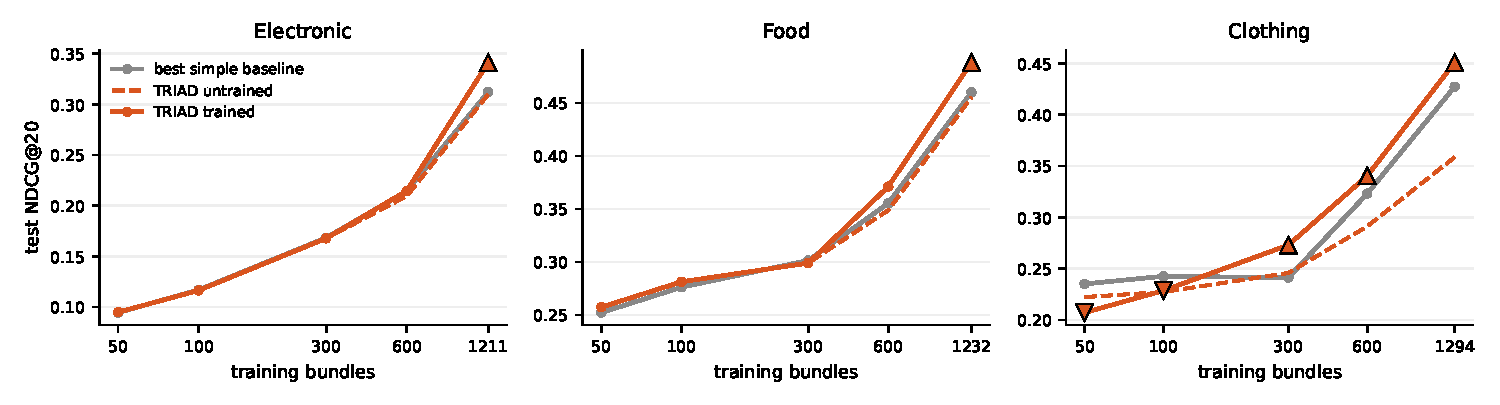
\includegraphics[width=\textwidth]{figs/training_size.pdf}
\caption{Test NDCG@20 against the number of training bundles (nested random subsets, three runs; baselines retuned
on each subset). Triangles: TRIAD significantly ahead ($\blacktriangle$) or behind ($\blacktriangledown$) the best
simple baseline, Holm over the 15 conditions.}
\label{fig:size}
\end{figure}

\begin{table}[!htb]
\centering
\caption{What each learned part is worth: validation NDCG@20 lost when one part is put back to its starting value
(or, for the shared exponent, $\alpha$ and $\beta$ replaced by their mean), as \% of the trained model, mean of three
runs. Measured on validation only (up to 1,000 queries per dataset). Bold: 5\% or more.}
\label{tab:knock}
\setlength{\tabcolsep}{2.2pt}
\scriptsize
\begin{tabular}{lccccccc}
\toprule
Part removed & Electr. & Food & Cloth. & POG\_D. & POG & Spot.\_s. & Spotify\\
\midrule
learned content maps ($M=$ start) & 1 & 0 & 2 & \textbf{19} & \textbf{59} & \textbf{11} & \textbf{8}\\
\quad antisymmetric part of $M_{zz}$ & 0 & 0 & 0 & \textbf{8} & \textbf{20} & 3 & 4\\
\quad partner histories ($M_{zh},M_{hz},M_{hh}=0$) & 1 & 0 & 0 & \textbf{12} & \textbf{22} & \textbf{7} & \textbf{6}\\
refined features ($z=x$) & 0 & $-$1 & 1 & \textbf{38} & \textbf{62} & \textbf{14} & \textbf{11}\\
label rule ($\delta_l=0$) & 1 & 1 & 2 & 2 & \textbf{14} & \textbf{47} & \textbf{29}\\
count exponents ($\alpha=\beta=\tfrac12$) & 3 & 3 & \textbf{7} & 3 & \textbf{8} & 2 & \textbf{31}\\
separate $\alpha,\beta$ (one shared value) & 0 & 0 & 0 & 0 & 0 & 0 & 0\\
popularity prior ($\rho=0$) & \textbf{13} & \textbf{10} & \textbf{15} & \textbf{56} & \textbf{50} & 5 & 1\\
gate (fixed at its mean weights) & 1 & 1 & 0 & 1 & 1 & \textbf{10} & \textbf{13}\\
\bottomrule
\end{tabular}
\end{table}

\paragraph{With little data, TRIAD stays at its starting heuristic.} We train TRIAD and retune the simple baselines on
nested random subsets of 50, 100, 300 and 600 training bundles (Fig.~\ref{fig:size}). With 50 to 300 bundles on
Electronic and Food, validation keeps the untrained model (epoch 0) in every run, so TRIAD equals its starting
heuristic and is level with the best simple baseline. With more bundles it moves away and pulls ahead. Over the 15
conditions TRIAD is significantly ahead in 5 and behind in 2 (Clothing with 50 and 100 bundles, where the label blend
is the best baseline and TRIAD's start, which has no label rule, is below it).

\paragraph{What TRIAD learns.} Every learned part is a function of a few inputs, so it can be read; Table~\ref{tab:knock}
shows what each is worth, on validation only. The domains use different parts.
\emph{Shared labels flip sign.} Since each term is divided by its largest value per query, only the sign of
$\delta_l$ and the ratios between its values affect a ranking. For one shared seed, $\delta_l$ is negative on outfits
in every run, 1.5 to 1.7 times more so for the largest categories than for the smallest (90th against 10th percentile
of label size), so a candidate in a seed's category leaves the shortlist. On playlists it is positive in every run,
and 2.9 to 3.7 times larger for an artist with one or two tracks than for one with 83 to 91. \emph{Outfits need fit, not similarity.} Measured by $\lVert M_{zz}-10I\rVert/\lVert10I\rVert$, $M_{zz}$ stays close to
its start on e-commerce (.10 to .17), while on outfits it moves by about its own size (1.01 to 1.09) and, among each item's ten nearest
neighbours, no longer agrees with cosine (correlation .19 on POG\_DENSE, $-$.17 on POG). Among the 100 highest-ranked candidates of each query, the partner-history blocks
carry 51\% to 69\% of the spread of the content score on outfits and playlists, against 8\% to 12\% on e-commerce. \emph{Popularity is evidence.} The candidate-side discount $\beta$ moves from $\tfrac12$ toward raw counts
on every dataset (.01 to .37), and the prior $\rho$, learned from training bundles only, follows the validation base
rate $b$ across frequency groups (correlation .96 to 1.00, .82 to .86 on Spotify; Clothing has only two groups). \emph{New seeds shift trust to
content.} For a query whose seeds were all never bundled, the gate raises the content weight by 36\% to 78\% on
e-commerce and playlists.

% =====================================================================================================================
\section{Conclusion}

We argued that bundle completion rests on relations between items that hold across the catalogue, rather than on a
representation of each item, and the data support this: many queries contain items that no training bundle holds, and
in outfits what goes together is not what is similar. TRIAD learns one scoring function over such relations, built as
a learnable family that contains the standard heuristics and starts at one of them. It is significantly ahead of the
tuned heuristics on all seven datasets and well above CLHE and RaMen, which learn a representation per item, on
identical splits. Its size does not depend on the catalogue, it stays at its starting heuristic when training data is
scarce, and its learned parameters show what each domain relies on: a shared category counts against a candidate in
outfits and a shared artist for it in playlists, outfits need fit rather than similarity, and popularity is evidence
to use, discounted far less than cosine normalization does.

\paragraph{Limitations.} With 50 and 100 training bundles on Clothing, TRIAD is behind a label-aware baseline. RaMen
on POG and Spotify and CLHE on full Spotify are published or single-run numbers. TRIAD sees an item only through its
pretrained features, labels and co-occurrence counts, so its content term is only as good as the features; on
e-commerce these come from item titles alone. Scoring is linear in the catalogue size, so millions of items would need
a candidate stage. Code will be released.

\begin{thebibliography}{99}\scriptsize
\bibitem{bgn} Bai, J., Zhou, C., Song, J., Qu, X., An, W., Li, Z., Gao, J.: Personalized bundle list recommendation. In: WWW (2019)
\bibitem{bgcn} Chang, J., Gao, C., He, X., Jin, D., Li, Y.: Bundle recommendation with graph convolutional networks. In: SIGIR (2020)
\bibitem{spotify} Chen, C.W., Lamere, P., Schedl, M., Zamani, H.: RecSys Challenge 2018: Automatic music playlist continuation. In: RecSys (2018)
\bibitem{pog} Chen, W., et al.: POG: Personalized outfit generation for fashion recommendation at Alibaba iFashion. In: KDD (2019)
\bibitem{link} Choi, M., Lee, S., Park, S., Lee, J.: Linear item-item model with neural knowledge for session-based recommendation. In: SIGIR (2025)
\bibitem{efron1993} Efron, B., Tibshirani, R.J.: An Introduction to the Bootstrap. Chapman \& Hall (1993)
\bibitem{dacrema} Ferrari Dacrema, M., Cremonesi, P., Jannach, D.: Are we really making much progress? A worrying analysis of recent neural recommendation approaches. In: RecSys (2019)
\bibitem{gartrell2017} Gartrell, M., Paquet, U., Koenigstein, N.: Low-rank factorization of determinantal point processes. In: AAAI (2017)
\bibitem{han2017} Han, X., Wu, Z., Jiang, Y.G., Davis, L.S.: Learning fashion compatibility with bidirectional LSTMs. In: ACM MM (2017)
\bibitem{lightgcn} He, X., Deng, K., Wang, X., Li, Y., Zhang, Y., Wang, M.: LightGCN: Simplifying and powering graph convolution network for recommendation. In: SIGIR (2020)
\bibitem{holm1979} Holm, S.: A simple sequentially rejective multiple test procedure. Scandinavian Journal of Statistics 6(2), 65--70 (1979)
\bibitem{hu2008} Hu, Y., Koren, Y., Volinsky, C.: Collaborative filtering for implicit feedback datasets. In: ICDM (2008)
\bibitem{kapoor2023} Kapoor, S., Narayanan, A.: Leakage and the reproducibility crisis in machine-learning-based science. Patterns 4(9) (2023)
\bibitem{krichene2020} Krichene, W., Rendle, S.: On sampled metrics for item recommendation. In: KDD (2020)
\bibitem{settransformer} Lee, J., Lee, Y., Kim, J., Kosiorek, A., Choi, S., Teh, Y.W.: Set Transformer: A framework for attention-based permutation-invariant neural networks. In: ICML (2019)
\bibitem{blip} Li, J., Li, D., Xiong, C., Hoi, S.: BLIP: Bootstrapping language-image pre-training for unified vision-language understanding and generation. In: ICML (2022)
\bibitem{bundlemllm} Liu, X., Wu, J., Tao, Z., Ma, Y., Wei, Y., Chua, T.S.: Fine-tuning multimodal large language models for product bundling. In: KDD (2025)
\bibitem{adamw} Loshchilov, I., Hutter, F.: Decoupled weight decay regularization. In: ICLR (2019)
\bibitem{crosscbr} Ma, Y., He, Y., Zhang, A., Wang, X., Chua, T.S.: CrossCBR: Cross-view contrastive learning for bundle recommendation. In: KDD (2022)
\bibitem{clhe} Ma, Y., Liu, X., Wei, Y., Tao, Z., Wang, X., Chua, T.S.: Leveraging multimodal features and item-level user feedback for bundle construction. In: WSDM (2024)
\bibitem{mcauley} McAuley, J., Pandey, R., Leskovec, J.: Inferring networks of substitutable and complementary products. In: KDD (2015)
\bibitem{ramen} Nguyen, H.S., Nguyen, Q.H., Pham, D.H., Le, D.T., Le, H.Q., Sitkrongwong, P., Takasu, A., Mansoury, M.: RaMen: Multi-strategy multi-modal learning for bundle construction. In: ECAI (2025)
\bibitem{caro} Nguyen, L.H., Nguyen, H.S., Nguyen, C.V.T., Le, D.T., Takasu, A., Le, H.Q.: Dual-enhanced item representation for bundle construction via category-wise and cross-modality learning. In: SIGIR-AP (2025)
\bibitem{rp3beta} Paudel, B., Christoffel, F., Newell, C., Bernstein, A.: Updatable, accurate, diverse, and scalable recommendations for interactive applications. ACM TiiS 7(1) (2017)
\bibitem{sgfcf} Peng, S., Liu, X., Sugiyama, K., Mine, T.: How powerful is graph filtering for recommendation. In: KDD (2024)
\bibitem{bpr} Rendle, S., Freudenthaler, C., Gantner, Z., Schmidt-Thieme, L.: BPR: Bayesian personalized ranking from implicit feedback. In: UAI (2009)
\bibitem{rendle2020} Rendle, S., Krichene, W., Zhang, L., Anderson, J.: Neural collaborative filtering vs. matrix factorization revisited. In: RecSys (2020)
\bibitem{sarwar2001} Sarwar, B., Karypis, G., Konstan, J., Riedl, J.: Item-based collaborative filtering recommendation algorithms. In: WWW (2001)
\bibitem{gfcf} Shen, Y., Wu, Y., Zhang, Y., Shan, C., Zhang, J., Letaief, K.B., Li, D.: How powerful is graph convolution for recommendation? In: CIKM (2021)
\bibitem{smucker2007} Smucker, M.D., Allan, J., Carterette, B.: A comparison of statistical significance tests for information retrieval evaluation. In: CIKM (2007)
\bibitem{steck2019} Steck, H.: Embarrassingly shallow autoencoders for sparse data. In: WWW (2019)
\bibitem{bundlerec} Sun, Z., Feng, K., Yang, J., Fang, H., Qu, X., Ong, Y.S., Liu, W.: Revisiting bundle recommendation for intent-aware product bundling. ACM TORS 2(3) (2024)
\bibitem{adabundle} Sun, Z., Feng, K., Yang, J., Qu, X., Fang, H., Ong, Y.S., Liu, W.: Adaptive in-context learning with large language models for bundle generation. In: SIGIR (2024)
\bibitem{ddbc} Tu, T., Li, A., Ma, Y., Xu, S., Liu, X., Ma, H., Pang, L., Chua, T.S.: Discrete diffusion for bundle construction. In: ICLR (2026)
\bibitem{vasileva2018} Vasileva, M.I., Plummer, B.A., Dusad, K., Rajpal, S., Kumar, R., Forsyth, D.: Learning type-aware embeddings for fashion compatibility. In: ECCV (2018)
\bibitem{clap} Wu, Y., Chen, K., Zhang, T., Hui, Y., Berg-Kirkpatrick, T., Dubnov, S.: Large-scale contrastive language-audio pretraining with feature fusion and keyword-to-caption augmentation. In: ICASSP (2023)
\bibitem{fashiondpo} Yu, M., Ma, Y., Wu, L., et al.: FashionDPO: Fine-tune fashion outfit generation model using direct preference optimization. In: SIGIR (2025)
\bibitem{deepsets} Zaheer, M., Kottur, S., Ravanbakhsh, S., Poczos, B., Salakhutdinov, R., Smola, A.: Deep sets. In: NeurIPS (2017)
\bibitem{nonmbb} Zhang, R., Wang, S., Jing, H., Liu, Y., Yao, Z.: Not all slots are equal: Non-co-progressive Markov bridge for bundle construction. In: NeurIPS (2026)
\end{thebibliography}
\end{document}
